\begin{itemize}
\tightlist
\item
  \textbf{\href{./}{Neuroanatomy}}
\item
\item
  \href{index.html}{\emph{}Welcome}
\item
  \href{acknowledgements.html}{\emph{}Acknowledgements}
\item
  \href{the-nervous-system.html}{\emph{}\textbf{1} The Nervous System}

  \begin{itemize}
  \tightlist
  \item
    \href{the-nervous-system.html\#introduction}{\emph{}\textbf{1.1}
    Introduction}
  \item
    \href{the-nervous-system.html\#the-cells-of-the-nervous-system}{\emph{}\textbf{1.2}
    The Cells Of The Nervous System}
  \item
    \href{the-nervous-system.html\#comparative-anatomy-and-evolution-of-nervous-systems}{\emph{}\textbf{1.3}
    Comparative Anatomy And Evolution Of Nervous Systems}
  \item
    \href{the-nervous-system.html\#the-human-brain}{\emph{}\textbf{1.4}
    The Human Brain}
  \item
    \href{the-nervous-system.html\#development-of-the-nervous-system}{\emph{}\textbf{1.5}
    Development Of The Nervous System}
  \item
    \href{the-nervous-system.html\#the-function-of-the-nervous-system}{\emph{}\textbf{1.6}
    The Function Of The Nervous System}
  \item
    \href{the-nervous-system.html\#the-sensory-system}{\emph{}\textbf{1.7}
    The Sensory System}
  \item
    \href{the-nervous-system.html\#the-motor-system}{\emph{}\textbf{1.8}
    The Motor System}
  \item
    \href{the-nervous-system.html\#neuronal-signalling}{\emph{}\textbf{1.9}
    Neuronal Signalling}
  \item
    \href{the-nervous-system.html\#neural-circuits}{\emph{}\textbf{1.10}
    Neural Circuits}
  \item
    \href{the-nervous-system.html\#reflexes-and-other-stimulus-response-circuits}{\emph{}\textbf{1.11}
    Reflexes And Other Stimulus-Response Circuits}
  \item
    \href{the-nervous-system.html\#intrinsic-pattern-generation}{\emph{}\textbf{1.12}
    Intrinsic Pattern Generation}
  \item
    \href{the-nervous-system.html\#neuroimaging}{\emph{}\textbf{1.13}
    Neuroimaging}

    \begin{itemize}
    \tightlist
    \item
      \href{the-nervous-system.html\#electroencephalography}{\emph{}\textbf{1.13.1}
      Electroencephalography}
    \item
      \href{the-nervous-system.html\#magnetoencephalography}{\emph{}\textbf{1.13.2}
      Magnetoencephalography}
    \item
      \href{the-nervous-system.html\#computed-axial-tomography}{\emph{}\textbf{1.13.3}
      Computed axial tomography}
    \item
      \href{the-nervous-system.html\#magnetic-resonance-imaging}{\emph{}\textbf{1.13.4}
      Magnetic resonance imaging}
    \item
      \href{the-nervous-system.html\#positron-emission-tomography}{\emph{}\textbf{1.13.5}
      Positron emission tomography}
    \item
      \href{the-nervous-system.html\#single-photon-emission-computed-tomography}{\emph{}\textbf{1.13.6}
      Single-photon emission computed tomography}
    \end{itemize}
  \end{itemize}
\item
  \href{development-of-the-nervous-system-1.html}{\emph{}\textbf{2}
  Development Of The Nervous System}

  \begin{itemize}
  \tightlist
  \item
    \href{development-of-the-nervous-system-1.html\#neural-induction}{\emph{}\textbf{2.1}
    Neural Induction}
  \item
    \href{development-of-the-nervous-system-1.html\#the-early-brain}{\emph{}\textbf{2.2}
    The Early Brain}
  \item
    \href{development-of-the-nervous-system-1.html\#patterning-of-the-nervous-system}{\emph{}\textbf{2.3}
    Patterning Of The Nervous System}
  \item
    \href{development-of-the-nervous-system-1.html\#neurogenesis}{\emph{}\textbf{2.4}
    Neurogenesis}
  \item
    \href{development-of-the-nervous-system-1.html\#neuronal-migration}{\emph{}\textbf{2.5}
    Neuronal Migration}
  \item
    \href{development-of-the-nervous-system-1.html\#neurotrophic-factors}{\emph{}\textbf{2.6}
    Neurotrophic Factors}
  \item
    \href{development-of-the-nervous-system-1.html\#activity-dependent-mechanisms-in-the-assembly-of-neural-circuits}{\emph{}\textbf{2.7}
    Activity Dependent Mechanisms In The Assembly Of Neural Circuits}
  \item
    \href{development-of-the-nervous-system-1.html\#critical-periods}{\emph{}\textbf{2.8}
    Critical Periods}

    \begin{itemize}
    \tightlist
    \item
      \href{development-of-the-nervous-system-1.html\#activity-dependent-competition}{\emph{}\textbf{2.8.1}
      Activity-dependent competition}
    \end{itemize}
  \item
    \href{development-of-the-nervous-system-1.html\#brain-plasticity}{\emph{}\textbf{2.9}
    Brain plasticity}
  \end{itemize}
\item
  \href{neurons-and-glial-cells.html}{\emph{}\textbf{3} Neurons And
  Glial Cells}

  \begin{itemize}
  \tightlist
  \item
    \href{neurons-and-glial-cells.html\#neurons}{\emph{}\textbf{3.1}
    Neurons}
  \item
    \href{neurons-and-glial-cells.html\#glia}{\emph{}\textbf{3.2} Glia}
  \end{itemize}
\item
  \href{electrical-basis-of-neuronal-function.html}{\emph{}\textbf{4}
  Electrical Basis Of Neuronal Function}

  \begin{itemize}
  \tightlist
  \item
    \href{electrical-basis-of-neuronal-function.html\#the-membrane-potential}{\emph{}\textbf{4.1}
    The Membrane Potential}
  \item
    \href{electrical-basis-of-neuronal-function.html\#ions-and-the-forces-driving-their-motion}{\emph{}\textbf{4.2}
    Ions And The Forces Driving Their Motion}
  \item
    \href{electrical-basis-of-neuronal-function.html\#the-plasma-membrane}{\emph{}\textbf{4.3}
    The Plasma Membrane}
  \item
    \href{electrical-basis-of-neuronal-function.html\#ion-pumps}{\emph{}\textbf{4.4}
    Ion Pumps}
  \item
    \href{electrical-basis-of-neuronal-function.html\#ion-channels}{\emph{}\textbf{4.5}
    Ion Channels}
  \item
    \href{electrical-basis-of-neuronal-function.html\#the-reversal-potential}{\emph{}\textbf{4.6}
    The Reversal Potential}
  \item
    \href{electrical-basis-of-neuronal-function.html\#the-resting-potential}{\emph{}\textbf{4.7}
    The Resting Potential}
  \item
    \href{electrical-basis-of-neuronal-function.html\#the-action-potential}{\emph{}\textbf{4.8}
    The Action Potential}
  \item
    \href{electrical-basis-of-neuronal-function.html\#graded-potentials}{\emph{}\textbf{4.9}
    Graded Potentials}
  \end{itemize}
\item
  \href{neurotransmission.html}{\emph{}\textbf{5} Neurotransmission}

  \begin{itemize}
  \tightlist
  \item
    \href{neurotransmission.html\#the-synapse}{\emph{}\textbf{5.1} The
    Synapse}
  \item
    \href{neurotransmission.html\#neurotransmitters}{\emph{}\textbf{5.2}
    Neurotransmitters}

    \begin{itemize}
    \tightlist
    \item
      \href{neurotransmission.html\#modulatory-neurotransmitter-systems}{\emph{}\textbf{5.2.1}
      Modulatory Neurotransmitter Systems}
    \end{itemize}
  \item
    \href{neurotransmission.html\#neurotransmitter-receptors}{\emph{}\textbf{5.3}
    Neurotransmitter Receptors}

    \begin{itemize}
    \tightlist
    \item
      \href{neurotransmission.html\#ionotropic-receptors-neurotransmitter-gated-ion-channels}{\emph{}\textbf{5.3.1}
      Ionotropic Receptors: Neurotransmitter-Gated Ion Channels}
    \item
      \href{neurotransmission.html\#metabotropic-receptors-g-protein-coupled-receptors}{\emph{}\textbf{5.3.2}
      Metabotropic Receptors: G-Protein Coupled Receptors}
    \end{itemize}
  \end{itemize}
\item
  \href{the-central-nervous-system.html}{\emph{}\textbf{6} The Central
  Nervous System}

  \begin{itemize}
  \tightlist
  \item
    \href{the-central-nervous-system.html\#the-meninges}{\emph{}\textbf{6.1}
    The Meninges}

    \begin{itemize}
    \tightlist
    \item
      \href{the-central-nervous-system.html\#dura-mater}{\emph{}\textbf{6.1.1}
      Dura Mater}
    \item
      \href{the-central-nervous-system.html\#arachnoid-mater}{\emph{}\textbf{6.1.2}
      Arachnoid Mater}
    \item
      \href{the-central-nervous-system.html\#pia-mater}{\emph{}\textbf{6.1.3}
      Pia Mater}
    \item
      \href{the-central-nervous-system.html\#subarachnoid-spaces}{\emph{}\textbf{6.1.4}
      Subarachnoid Spaces}
    \end{itemize}
  \item
    \href{the-central-nervous-system.html\#the-ventricular-system}{\emph{}\textbf{6.2}
    The Ventricular System}
  \item
    \href{the-central-nervous-system.html\#the-cerebrospinal-fluid}{\emph{}\textbf{6.3}
    The Cerebrospinal Fluid}
  \item
    \href{the-central-nervous-system.html\#the-blood-brain-barrier}{\emph{}\textbf{6.4}
    The Blood-Brain-Barrier}

    \begin{itemize}
    \tightlist
    \item
      \href{the-central-nervous-system.html\#circumventricular-organs}{\emph{}\textbf{6.4.1}
      Circumventricular Organs}
    \end{itemize}
  \item
    \href{the-central-nervous-system.html\#the-cerebrum}{\emph{}\textbf{6.5}
    The Cerebrum}

    \begin{itemize}
    \tightlist
    \item
      \href{the-central-nervous-system.html\#the-cerebral-cortex}{\emph{}\textbf{6.5.1}
      The Cerebral Cortex}
    \item
      \href{the-central-nervous-system.html\#the-basal-ganglia}{\emph{}\textbf{6.5.2}
      The Basal Ganglia}
    \item
      \href{the-central-nervous-system.html\#the-limbic-lobe}{\emph{}\textbf{6.5.3}
      The Limbic Lobe}
    \item
      \href{the-central-nervous-system.html\#the-hippocampus}{\emph{}\textbf{6.5.4}
      The Hippocampus}
    \item
      \href{the-central-nervous-system.html\#the-amygdala}{\emph{}\textbf{6.5.5}
      The Amygdala}
    \item
      \href{the-central-nervous-system.html\#the-thalamus}{\emph{}\textbf{6.5.6}
      The Thalamus}
    \item
      \href{the-central-nervous-system.html\#the-hypothalamus}{\emph{}\textbf{6.5.7}
      The Hypothalamus}
    \item
      \href{the-central-nervous-system.html\#the-brainstem}{\emph{}\textbf{6.5.8}
      The Brainstem}
    \item
      \href{the-central-nervous-system.html\#the-midbrain}{\emph{}\textbf{6.5.9}
      The Midbrain}
    \item
      \href{the-central-nervous-system.html\#the-cerebellum}{\emph{}\textbf{6.5.10}
      The Cerebellum}
    \end{itemize}
  \item
    \href{the-central-nervous-system.html\#the-spinal-cord}{\emph{}\textbf{6.6}
    The Spinal cord}
  \item
    \href{the-central-nervous-system.html\#central-neural-pathways}{\emph{}\textbf{6.7}
    Central Neural Pathways}

    \begin{itemize}
    \tightlist
    \item
      \href{the-central-nervous-system.html\#the-corpus-callosum}{\emph{}\textbf{6.7.1}
      The Corpus Callosum}
    \item
      \href{the-central-nervous-system.html\#the-cerebral-peduncles}{\emph{}\textbf{6.7.2}
      The Cerebral Peduncles}
    \item
      \href{the-central-nervous-system.html\#the-pyramidal-tracts}{\emph{}\textbf{6.7.3}
      The Pyramidal Tracts}
    \item
      \href{the-central-nervous-system.html\#the-corticopontine-fibers}{\emph{}\textbf{6.7.4}
      The Corticopontine Fibers}
    \item
      \href{the-central-nervous-system.html\#the-spinal-tracts}{\emph{}\textbf{6.7.5}
      The Spinal Tracts}
    \item
      \href{the-central-nervous-system.html\#the-spinocerebellar-tracts}{\emph{}\textbf{6.7.6}
      The Spinocerebellar Tracts}
    \item
      \href{the-central-nervous-system.html\#default-mode-network}{\emph{}\textbf{6.7.7}
      Default mode network}
    \end{itemize}
  \item
    \href{the-central-nervous-system.html\#sensory-maps}{\emph{}\textbf{6.8}
    Sensory Maps}
  \item
    \href{the-central-nervous-system.html\#the-cortical-homunculus}{\emph{}\textbf{6.9}
    The Cortical Homunculus}
  \end{itemize}
\item
  \href{the-peripheral-nervous-system.html}{\emph{}\textbf{7} The
  Peripheral Nervous System}

  \begin{itemize}
  \tightlist
  \item
    \href{the-peripheral-nervous-system.html\#the-somatic-nervous-system}{\emph{}\textbf{7.1}
    The Somatic Nervous System}
  \item
    \href{the-peripheral-nervous-system.html\#the-cranial-nerves}{\emph{}\textbf{7.2}
    The Cranial Nerves}

    \begin{itemize}
    \tightlist
    \item
      \href{the-peripheral-nervous-system.html\#smell-i}{\emph{}\textbf{7.2.1}
      Smell (I)}
    \item
      \href{the-peripheral-nervous-system.html\#vision-ii}{\emph{}\textbf{7.2.2}
      Vision (II)}
    \item
      \href{the-peripheral-nervous-system.html\#eye-movement-iii-iv-vi}{\emph{}\textbf{7.2.3}
      Eye movement (III, IV, VI)}
    \item
      \href{the-peripheral-nervous-system.html\#trigeminal-nerve-v}{\emph{}\textbf{7.2.4}
      Trigeminal nerve (V)}
    \item
      \href{the-peripheral-nervous-system.html\#facial-expression-vii}{\emph{}\textbf{7.2.5}
      Facial expression (VII)}
    \item
      \href{the-peripheral-nervous-system.html\#hearing-and-balance-viii}{\emph{}\textbf{7.2.6}
      Hearing and balance (VIII)}
    \item
      \href{the-peripheral-nervous-system.html\#oral-sensation-taste-and-salivation-ix}{\emph{}\textbf{7.2.7}
      Oral Sensation, Taste, And Salivation (Ix)}
    \item
      \href{the-peripheral-nervous-system.html\#vagus-nerve-x}{\emph{}\textbf{7.2.8}
      Vagus Nerve (X)}
    \item
      \href{the-peripheral-nervous-system.html\#shoulder-elevation-and-head-turning-xi}{\emph{}\textbf{7.2.9}
      Shoulder Elevation And Head-Turning (XI)}
    \item
      \href{the-peripheral-nervous-system.html\#tongue-movement-xii}{\emph{}\textbf{7.2.10}
      Tongue Movement (XII)}
    \end{itemize}
  \item
    \href{the-peripheral-nervous-system.html\#the-spinal-nerves}{\emph{}\textbf{7.3}
    The Spinal Nerves}

    \begin{itemize}
    \tightlist
    \item
      \href{the-peripheral-nervous-system.html\#cervical-spinal-nerves-c1c4}{\emph{}\textbf{7.3.1}
      Cervical Spinal Nerves (C1--C4)}
    \item
      \href{the-peripheral-nervous-system.html\#brachial-plexus-c5t1}{\emph{}\textbf{7.3.2}
      Brachial Plexus (C5--T1)}
    \item
      \href{the-peripheral-nervous-system.html\#lumbosacral-plexus-l1co1}{\emph{}\textbf{7.3.3}
      Lumbosacral Plexus (L1--Co1)}
    \end{itemize}
  \item
    \href{the-peripheral-nervous-system.html\#the-autonomic-nervous-system}{\emph{}\textbf{7.4}
    The Autonomic Nervous System}
  \item
    \href{the-peripheral-nervous-system.html\#the-sympathetic-nervous-system}{\emph{}\textbf{7.5}
    The Sympathetic Nervous System}
  \item
    \href{the-peripheral-nervous-system.html\#the-parasympathetic-nervous-system}{\emph{}\textbf{7.6}
    The Parasympathetic Nervous System}
  \end{itemize}
\item
  \href{the-somatic-sensory-system.html}{\emph{}\textbf{8} The Somatic
  Sensory System}

  \begin{itemize}
  \tightlist
  \item
    \href{the-somatic-sensory-system.html\#touch}{\emph{}\textbf{8.1}
    Touch}
  \item
    \href{the-somatic-sensory-system.html\#cutaneous-mechanoreceptors}{\emph{}\textbf{8.2}
    Cutaneous Mechanoreceptors}
  \item
    \href{the-somatic-sensory-system.html\#nociception}{\emph{}\textbf{8.3}
    Nociception}
  \item
    \href{the-somatic-sensory-system.html\#proprioception}{\emph{}\textbf{8.4}
    Proprioception}
  \item
    \href{the-somatic-sensory-system.html\#muscle-spindles}{\emph{}\textbf{8.5}
    Muscle Spindles}
  \item
    \href{the-somatic-sensory-system.html\#golgi-tendon-organ}{\emph{}\textbf{8.6}
    Golgi Tendon Organ}
  \item
    \href{the-somatic-sensory-system.html\#the-somatosensory-pathways}{\emph{}\textbf{8.7}
    The Somatosensory Pathways}
  \item
    \href{the-somatic-sensory-system.html\#the-primary-somatosensory-cortex}{\emph{}\textbf{8.8}
    The Primary Somatosensory Cortex}
  \end{itemize}
\item
  \href{the-visual-system.html}{\emph{}\textbf{9} The Visual System}

  \begin{itemize}
  \tightlist
  \item
    \href{the-visual-system.html\#the-eye}{\emph{}\textbf{9.1} The Eye}
  \item
    \href{the-visual-system.html\#the-retina}{\emph{}\textbf{9.2} The
    Retina}
  \item
    \href{the-visual-system.html\#the-photoreceptors}{\emph{}\textbf{9.3}
    The Photoreceptors}
  \item
    \href{the-visual-system.html\#visual-phototransduction}{\emph{}\textbf{9.4}
    Visual Phototransduction}
  \item
    \href{the-visual-system.html\#the-visual-pathways}{\emph{}\textbf{9.5}
    The Visual Pathways}

    \begin{itemize}
    \tightlist
    \item
      \href{the-visual-system.html\#the-optic-nerve-and-optic-tract}{\emph{}\textbf{9.5.1}
      The Optic Nerve And Optic Tract}
    \end{itemize}
  \item
    \href{the-visual-system.html\#the-superior-colliculus}{\emph{}\textbf{9.6}
    The Superior Colliculus}
  \item
    \href{the-visual-system.html\#the-lateral-geniculate-nucleus-lgn}{\emph{}\textbf{9.7}
    The Lateral Geniculate Nucleus (LGN)}
  \item
    \href{the-visual-system.html\#the-visual-cortex}{\emph{}\textbf{9.8}
    The Visual Cortex}
  \end{itemize}
\item
  \href{the-auditory-and-vestibular-systems.html}{\emph{}\textbf{10} The
  Auditory And Vestibular Systems}

  \begin{itemize}
  \tightlist
  \item
    \href{the-auditory-and-vestibular-systems.html\#the-ear}{\emph{}\textbf{10.1}
    The Ear}
  \item
    \href{the-auditory-and-vestibular-systems.html\#the-auditory-system}{\emph{}\textbf{10.2}
    The Auditory System}

    \begin{itemize}
    \tightlist
    \item
      \href{the-auditory-and-vestibular-systems.html\#organ-of-corti}{\emph{}\textbf{10.2.1}
      Organ Of Corti}
    \item
      \href{the-auditory-and-vestibular-systems.html\#auditory-transduction}{\emph{}\textbf{10.2.2}
      Auditory Transduction}
    \item
      \href{the-auditory-and-vestibular-systems.html\#auditory-pathways}{\emph{}\textbf{10.2.3}
      Auditory Pathways}
    \item
      \href{the-auditory-and-vestibular-systems.html\#the-cochlear-nucleus}{\emph{}\textbf{10.2.4}
      The Cochlear Nucleus}
    \item
      \href{the-auditory-and-vestibular-systems.html\#the-trapezoid-body}{\emph{}\textbf{10.2.5}
      The Trapezoid Body}
    \item
      \href{the-auditory-and-vestibular-systems.html\#the-superior-olivary-complex}{\emph{}\textbf{10.2.6}
      The superior olivary complex}
    \item
      \href{the-auditory-and-vestibular-systems.html\#the-lateral-lemniscus}{\emph{}\textbf{10.2.7}
      The Lateral Lemniscus}
    \item
      \href{the-auditory-and-vestibular-systems.html\#the-inferior-colliculi}{\emph{}\textbf{10.2.8}
      The Inferior Colliculi}
    \item
      \href{the-auditory-and-vestibular-systems.html\#the-medial-geniculate-nucleus-mgn}{\emph{}\textbf{10.2.9}
      The Medial Geniculate Nucleus (MGN)}
    \item
      \href{the-auditory-and-vestibular-systems.html\#the-primary-auditory-cortex}{\emph{}\textbf{10.2.10}
      The Primary Auditory Cortex}
    \item
      \href{the-auditory-and-vestibular-systems.html\#the-auditory-ventral-and-dorsal-streams}{\emph{}\textbf{10.2.11}
      The Auditory Ventral And Dorsal Streams}
    \end{itemize}
  \item
    \href{the-auditory-and-vestibular-systems.html\#the-vestibular-system}{\emph{}\textbf{10.3}
    The Vestibular System}

    \begin{itemize}
    \tightlist
    \item
      \href{the-auditory-and-vestibular-systems.html\#the-semicircular-canals}{\emph{}\textbf{10.3.1}
      The Semicircular Canals}
    \item
      \href{the-auditory-and-vestibular-systems.html\#the-otolithic-organs}{\emph{}\textbf{10.3.2}
      The Otolithic Organs}
    \item
      \href{the-auditory-and-vestibular-systems.html\#vestibular-pathways}{\emph{}\textbf{10.3.3}
      Vestibular Pathways}
    \end{itemize}
  \end{itemize}
\item
  \href{the-olfactory-system.html}{\emph{}\textbf{11} The Olfactory
  System}

  \begin{itemize}
  \tightlist
  \item
    \href{the-olfactory-system.html\#the-nose}{\emph{}\textbf{11.1} The
    Nose}
  \item
    \href{the-olfactory-system.html\#olfactory-sensory-neurons}{\emph{}\textbf{11.2}
    Olfactory Sensory Neurons}
  \item
    \href{the-olfactory-system.html\#the-olfactory-bulb}{\emph{}\textbf{11.3}
    The Olfactory Bulb}
  \item
    \href{the-olfactory-system.html\#the-olfactory-cortex}{\emph{}\textbf{11.4}
    The Olfactory Cortex}
  \item
    \href{the-olfactory-system.html\#olfactory-pathways}{\emph{}\textbf{11.5}
    Olfactory Pathways}
  \end{itemize}
\item
  \href{the-gustatory-system.html}{\emph{}\textbf{12} The Gustatory
  System}

  \begin{itemize}
  \tightlist
  \item
    \href{the-gustatory-system.html\#the-tongue}{\emph{}\textbf{12.1}
    The Tongue}
  \item
    \href{the-gustatory-system.html\#the-five-basic-tastes}{\emph{}\textbf{12.2}
    The Five Basic Tastes}

    \begin{itemize}
    \tightlist
    \item
      \href{the-gustatory-system.html\#sweetness}{\emph{}\textbf{12.2.1}
      Sweetness}
    \item
      \href{the-gustatory-system.html\#sourness}{\emph{}\textbf{12.2.2}
      Sourness}
    \item
      \href{the-gustatory-system.html\#saltiness}{\emph{}\textbf{12.2.3}
      Saltiness}
    \item
      \href{the-gustatory-system.html\#bitterness}{\emph{}\textbf{12.2.4}
      Bitterness}
    \item
      \href{the-gustatory-system.html\#savoriness-umami}{\emph{}\textbf{12.2.5}
      Savoriness (Umami)}
    \end{itemize}
  \item
    \href{the-gustatory-system.html\#the-taste-receptors}{\emph{}\textbf{12.3}
    The Taste Receptors}
  \item
    \href{the-gustatory-system.html\#the-gustatory-nucleus}{\emph{}\textbf{12.4}
    The Gustatory Nucleus}
  \item
    \href{the-gustatory-system.html\#the-gustatory-cortex}{\emph{}\textbf{12.5}
    The Gustatory Cortex}
  \end{itemize}
\item
  \href{the-somatic-motor-system.html}{\emph{}\textbf{13} The Somatic
  Motor System}

  \begin{itemize}
  \tightlist
  \item
    \href{the-somatic-motor-system.html\#skeletal-muscle}{\emph{}\textbf{13.1}
    Skeletal Muscle}
  \item
    \href{the-somatic-motor-system.html\#the-muscle-fiber}{\emph{}\textbf{13.2}
    The Muscle Fiber}
  \item
    \href{the-somatic-motor-system.html\#the-motor-unit}{\emph{}\textbf{13.3}
    The Motor Unit}
  \item
    \href{the-somatic-motor-system.html\#somatic-motor-neurons}{\emph{}\textbf{13.4}
    Somatic Motor Neurons}
  \item
    \href{the-somatic-motor-system.html\#neuromuscular-junction}{\emph{}\textbf{13.5}
    Neuromuscular Junction}

    \begin{itemize}
    \tightlist
    \item
      \href{the-somatic-motor-system.html\#muscle-contraction}{\emph{}\textbf{13.5.1}
      Muscle Contraction}
    \item
      \href{the-somatic-motor-system.html\#sliding-filament-theory}{\emph{}\textbf{13.5.2}
      Sliding filament theory}
    \item
      \href{the-somatic-motor-system.html\#crossbridge-cycling}{\emph{}\textbf{13.5.3}
      Crossbridge cycling}
    \item
      \href{the-somatic-motor-system.html\#the-stretch-reflex}{\emph{}\textbf{13.5.4}
      The Stretch Reflex}
    \end{itemize}
  \item
    \href{the-somatic-motor-system.html\#the-motor-cortex}{\emph{}\textbf{13.6}
    The Motor Cortex}

    \begin{itemize}
    \tightlist
    \item
      \href{the-somatic-motor-system.html\#the-supplementary-motor-cortex}{\emph{}\textbf{13.6.1}
      The Supplementary Motor Cortex}
    \end{itemize}
  \item
    \href{the-somatic-motor-system.html\#the-basal-ganglia-1}{\emph{}\textbf{13.7}
    The Basal Ganglia}
  \item
    \href{the-somatic-motor-system.html\#the-cortico-basal-ganglia-thalamo-cortical-loop}{\emph{}\textbf{13.8}
    The Cortico-Basal Ganglia-Thalamo-Cortical Loop}
  \item
    \href{the-somatic-motor-system.html\#the-pyramidal-motor-system}{\emph{}\textbf{13.9}
    The Pyramidal Motor System}

    \begin{itemize}
    \tightlist
    \item
      \href{the-somatic-motor-system.html\#the-corticospinal-tract-1}{\emph{}\textbf{13.9.1}
      The Corticospinal Tract}
    \item
      \href{the-somatic-motor-system.html\#the-corticobulbar-tract-1}{\emph{}\textbf{13.9.2}
      The Corticobulbar Tract}
    \end{itemize}
  \item
    \href{the-somatic-motor-system.html\#the-extrapyramidal-motor-system}{\emph{}\textbf{13.10}
    The Extrapyramidal Motor System}
  \end{itemize}
\item
  \href{major-diseases-of-the-nervous-system.html}{\emph{}\textbf{14}
  Major Diseases Of The Nervous System}

  \begin{itemize}
  \tightlist
  \item
    \href{major-diseases-of-the-nervous-system.html\#neurodegenerative-diseases}{\emph{}\textbf{14.1}
    Neurodegenerative Diseases}

    \begin{itemize}
    \tightlist
    \item
      \href{major-diseases-of-the-nervous-system.html\#alzheimers-disease}{\emph{}\textbf{14.1.1}
      Alzheimer's disease}
    \item
      \href{major-diseases-of-the-nervous-system.html\#parkinsons-disease}{\emph{}\textbf{14.1.2}
      Parkinson's disease}
    \item
      \href{major-diseases-of-the-nervous-system.html\#huntingtons-disease}{\emph{}\textbf{14.1.3}
      Huntington's disease}
    \item
      \href{major-diseases-of-the-nervous-system.html\#amyotrophic-lateral-sclerosis-als}{\emph{}\textbf{14.1.4}
      Amyotrophic lateral sclerosis (ALS)}
    \end{itemize}
  \item
    \href{major-diseases-of-the-nervous-system.html\#cerebrovascular-disease}{\emph{}\textbf{14.2}
    Cerebrovascular Disease}

    \begin{itemize}
    \tightlist
    \item
      \href{major-diseases-of-the-nervous-system.html\#stroke}{\emph{}\textbf{14.2.1}
      Stroke}
    \item
      \href{major-diseases-of-the-nervous-system.html\#aphasia}{\emph{}\textbf{14.2.2}
      Aphasia}
    \item
      \href{major-diseases-of-the-nervous-system.html\#prosopagnosia}{\emph{}\textbf{14.2.3}
      Prosopagnosia}
    \item
      \href{major-diseases-of-the-nervous-system.html\#hemispatial-neglect}{\emph{}\textbf{14.2.4}
      Hemispatial neglect}
    \end{itemize}
  \item
    \href{major-diseases-of-the-nervous-system.html\#epilepsy}{\emph{}\textbf{14.3}
    Epilepsy}
  \item
    \href{major-diseases-of-the-nervous-system.html\#mental-disorders}{\emph{}\textbf{14.4}
    Mental Disorders}

    \begin{itemize}
    \tightlist
    \item
      \href{major-diseases-of-the-nervous-system.html\#mood-disorders}{\emph{}\textbf{14.4.1}
      Mood Disorders}
    \item
      \href{major-diseases-of-the-nervous-system.html\#schizophrenia}{\emph{}\textbf{14.4.2}
      Schizophrenia}
    \end{itemize}
  \end{itemize}
\item
  {\textbf{Appendix}}
\item
  \href{anatomical-terms-of-location.html}{\emph{}\textbf{A} Anatomical
  Terms Of Location}

  \begin{itemize}
  \tightlist
  \item
    \href{anatomical-terms-of-location.html\#anatomical-planes}{\emph{}\textbf{A.1}
    Anatomical Planes}
  \item
    \href{anatomical-terms-of-location.html\#anatomical-axes}{\emph{}\textbf{A.2}
    Anatomical Axes}
  \item
    \href{anatomical-terms-of-location.html\#main-anatomical-terms}{\emph{}\textbf{A.3}
    Main Anatomical Terms}

    \begin{itemize}
    \tightlist
    \item
      \href{anatomical-terms-of-location.html\#superior-and-inferior}{\emph{}\textbf{A.3.1}
      Superior And Inferior}
    \item
      \href{anatomical-terms-of-location.html\#anterior-and-posterior}{\emph{}\textbf{A.3.2}
      Anterior And Posterior}
    \item
      \href{anatomical-terms-of-location.html\#medial-and-lateral}{\emph{}\textbf{A.3.3}
      Medial And Lateral}
    \item
      \href{anatomical-terms-of-location.html\#central-and-peripheral}{\emph{}\textbf{A.3.4}
      Central And Peripheral}
    \item
      \href{anatomical-terms-of-location.html\#superficial-and-deep}{\emph{}\textbf{A.3.5}
      Superficial And Deep}
    \item
      \href{anatomical-terms-of-location.html\#dorsal-and-ventral}{\emph{}\textbf{A.3.6}
      Dorsal And Ventral}
    \item
      \href{anatomical-terms-of-location.html\#cranial-and-caudal}{\emph{}\textbf{A.3.7}
      Cranial And Caudal}
    \end{itemize}
  \item
    \href{anatomical-terms-of-location.html\#prefixes}{\emph{}\textbf{A.4}
    Prefixes}
  \end{itemize}
\item
  \href{neuroanatomical-terms.html}{\emph{}\textbf{B} Neuroanatomical
  Terms}

  \begin{itemize}
  \tightlist
  \item
    \href{neuroanatomical-terms.html\#nucleus}{\emph{}\textbf{B.1}
    Nucleus}
  \item
    \href{neuroanatomical-terms.html\#ganglion}{\emph{}\textbf{B.2}
    Ganglion}
  \item
    \href{neuroanatomical-terms.html\#tract}{\emph{}\textbf{B.3} Tract}
  \item
    \href{neuroanatomical-terms.html\#lemniscus}{\emph{}\textbf{B.4}
    Lemniscus}
  \end{itemize}
\item
  \href{list-of-regions-in-the-human-brain.html}{\emph{}\textbf{C} List
  Of Regions In The Human Brain}

  \begin{itemize}
  \tightlist
  \item
    \href{list-of-regions-in-the-human-brain.html\#hindbrain-rhombencephalon}{\emph{}\textbf{C.1}
    Hindbrain (rhombencephalon)}
  \item
    \href{list-of-regions-in-the-human-brain.html\#midbrain-mesencephalon}{\emph{}\textbf{C.2}
    Midbrain (mesencephalon)}
  \item
    \href{list-of-regions-in-the-human-brain.html\#forebrain-prosencephalon}{\emph{}\textbf{C.3}
    Forebrain (prosencephalon)}
  \end{itemize}
\item
  \href{neural-pathways.html}{\emph{}\textbf{D} Neural pathways}

  \begin{itemize}
  \tightlist
  \item
    \href{neural-pathways.html\#motor-systems-descending-fibers}{\emph{}\textbf{D.1}
    Motor systems / Descending fibers}
  \item
    \href{neural-pathways.html\#somatosensory-system}{\emph{}\textbf{D.2}
    Somatosensory system}
  \item
    \href{neural-pathways.html\#visual-system}{\emph{}\textbf{D.3}
    Visual system}
  \item
    \href{neural-pathways.html\#auditory-system}{\emph{}\textbf{D.4}
    Auditory system}
  \end{itemize}
\item
  \href{brodmann-areas.html}{\emph{}\textbf{E} Brodmann Areas}
\end{itemize}

\hypertarget{text-for-bio400-neuroanatomy-at-salem-state-university}{%
\section{\texorpdfstring{\emph{}\href{./}{Text For BIO400 Neuroanatomy
at Salem State
University}}{Text For BIO400 Neuroanatomy at Salem State University}}\label{text-for-bio400-neuroanatomy-at-salem-state-university}}

\hypertarget{section-}{}
\hypertarget{the-somatic-motor-system}{%
\section{\texorpdfstring{{13} The Somatic Motor
System}{13 The Somatic Motor System}}\label{the-somatic-motor-system}}

The somatic motor system (SMS or voluntary nervous system) is the part
of the central and peripheral nervous system associated with the
voluntary control of body movements via skeletal muscles.

The somatic nervous system consists of afferent nerves or sensory
nerves, and efferent nerves or motor nerves and neurons in the brain and
spinal cord. Afferent nerves are responsible for relaying sensation from
the body to the central nervous system; efferent nerves are responsible
for sending out commands from the CNS to the body, stimulating muscle
contraction; they include all the non-sensory neurons connected with
skeletal muscles and skin. The a- of afferent and the e- of efferent
correspond to the prefixes ad- (to, toward) and ex- (out of).

Peripheral structures of the somatic motor system include skeletal
muscles and neural connections with muscle tissues. Central structures
include cerebral cortex, brainstem, spinal cord, pyramidal system
including the upper motor neurons, extrapyramidal system, cerebellum,
and the lower motor neurons in the brainstem and the spinal cord.

\hypertarget{skeletal-muscle}{%
\subsection{\texorpdfstring{{13.1} Skeletal
Muscle}{13.1 Skeletal Muscle}}\label{skeletal-muscle}}

Skeletal muscle is one of three major muscle types, the others being
cardiac muscle and smooth muscle. It is a form of striated muscle
tissue, which is under the voluntary control of the somatic nervous
system. Most skeletal muscles are attached to bones by bundles of
collagen fibers known as tendons.

Many muscles are named by the action the muscle performs. These include:

The flexor and extensor; abductor and adductor; levator and depressor;
supinator and pronator; sphincter, tensor, and rotator muscles.

A flexor muscle decreases the anterior angle at a joint; an extensor
increases the anterior angle at a joint.

An abductor moves a bone away from the midline; an adductor moves a bone
closer to the midline.

A levator raises a structure; a depressor moves a structure down.

A supinator turns the palm of the hand up; a pronator turns the palm
down.

A sphincter decreases the size of an opening; a tensor tenses a body
part; a rotator turns a bone around its axis.

René Descartes (1596--1650) was one of the first to conceive a model of
reciprocal innervation (in 1626) as the principle that provides for the
control of agonist and antagonist muscles. Reciprocal innervation
describes skeletal muscles as existing in antagonistic pairs, with
contraction of one muscle producing forces opposite to those generated
by contraction of the other. For example, in the human arm, the triceps
acts to extend the lower arm outward while the biceps acts to flex the
lower arm inward. To reach optimum efficiency, contraction of opposing
muscles must be inhibited while muscles with the desired action are
excited. This reciprocal innervation occurs so that the contraction of a
muscle results in the simultaneous relaxation of its corresponding
antagonist.

A common example of reciprocal innervation, is the effect of the
nociceptive (or nocifensive) reflex, or defensive response to pain,
otherwise commonly known as the withdrawal reflex; a type of involuntary
action of the body to remove the body part from the vicinity of an
offending object by contracting the appropriate muscles (usually flexor
muscles), while relaxing the extensor muscles.

The concept of reciprocal innervation is also applicable to the eye
(Sherrington's law), wherein increased innervation to an extraocular
muscle is accompanied by a simultaneous decrease in innervation to its
specific antagonist, such as the medial rectus and the lateral rectus in
the case of an eye looking to one side of the midline. When looking
outward or laterally, the lateral rectus of one eye must contract via
increased innervation, while its antagonist, the medial rectus of the
same eye - shall relax. The converse would occur in the other eye.

\hypertarget{the-muscle-fiber}{%
\subsection{\texorpdfstring{{13.2} The Muscle
Fiber}{13.2 The Muscle Fiber}}\label{the-muscle-fiber}}

A skeletal muscle refers to multiple bundles (fascicles) of cells joined
together called muscle fibers. The fibers and muscles are surrounded by
connective tissue layers called fasciae. Muscle fibers, or muscle cells,
are formed from the fusion of developmental myoblasts in a process known
as myogenesis. Muscle fibers are cylindrical and have more than one
nucleus.

\protect\hypertarget{fig:muscle}{}{}
\includegraphics[width=0.7\textwidth,height=\textheight]{figures/motor/1022_Muscle_Fibers_(small).jpg}

Figure 13.1:
\href{https://upload.wikimedia.org/wikipedia/commons/9/9c/1022_Muscle_Fibers_\%28small\%29.jpg}{Structure
of the skeletal muscle fiber.}

Muscle fibers are in turn composed of myofibrils. The myofibrils are
composed of actin and myosin filaments, repeated in units called
sarcomeres, which are the basic functional units of the muscle fiber.
The sarcomere is responsible for the striated appearance of skeletal
muscle and forms the basic machinery necessary for muscle contraction.

Every single organelle and macromolecule of a muscle fiber is arranged
to ensure form meets function. The cell membrane is called the
sarcolemma with the cytoplasm known as the sarcoplasm. In the sarcoplasm
are the myofibrils. The myofibrils are long protein bundles about 1
micrometer in diameter each containing myofilaments. Pressed against the
inside of the sarcolemma are the unusual flattened myonuclei. Between
the myofibrils are the mitochondria.

While the muscle fiber does not have smooth endoplasmic cisternae, it
contains a sarcoplasmic reticulum. The sarcoplasmic reticulum surrounds
the myofibrils and holds a reserve of the calcium ions needed to cause a
muscle contraction. Periodically, it has dilated end sacs known as
terminal cisternae. These cross the muscle fiber from one side to the
other. In between two terminal cisternae is a tubular infolding called a
transverse tubule (T tubule). T tubules are the pathways for action
potentials to signal the sarcoplasmic reticulum to release calcium,
causing a muscle contraction. Together, two terminal cisternae and a
transverse tubule form a triad.

In addition to the actin and myosin components that constitute the
sarcomere, skeletal muscle fibers also contain two other important
regulatory proteins, troponin and tropomyosin, that are necessary for
muscle contraction to occur. These proteins are associated with actin
and cooperate to prevent its interaction with myosin.

Once a cell is sufficiently stimulated, the cell's sarcoplasmic
reticulum releases ionic calcium (Ca\textsuperscript{2+}), which then
interacts with the regulatory protein troponin. Calcium-bound troponin
undergoes a conformational change that leads to the movement of
tropomyosin, subsequently exposing the myosin-binding sites on actin.
This allows for myosin and actin ATP-dependent cross-bridge cycling and
shortening of the muscle.

\protect\hypertarget{fig:sercastructure}{}{}
\includegraphics[width=0.7\textwidth,height=\textheight]{figures/motor/Ca_pump.png}

Figure 13.2: A cartoon representation of the crystal structure of the
Ca\textsuperscript{2+} pump of the skeletal muscle sarcoplasmic
reticulum. Atomic coordinates of
\href{https://www.rcsb.org/structure/1VFP}{PDB 1VFP}, rendered with open
source molecular visualization tool PyMol.

\hypertarget{the-motor-unit}{%
\subsection{\texorpdfstring{{13.3} The Motor
Unit}{13.3 The Motor Unit}}\label{the-motor-unit}}

Motor units are multiple muscle fibers bundled together. When a person
wants to move their body to achieve a certain task, the brain sends an
impulse signal that reaches the specific motor unit through the spinal
cord. After receiving the signal from the brain, the motor unit
contracts muscle fibers within the group to create movement. There is no
partial firing in the motor unit, meaning, once the signal is detected,
all the muscles fibers within the unit contract. However, there are
different intensities. Since each motor unit contracts 100\% of its
fiber once stimulated, types of motor units that generate different
force or speed are significant.

For low intensity tasks, smaller motor units with fewer muscle fibers
are used. These smaller motor units are known as low threshold motor
units. They consist of type I fibers that contract much slower and thus
provide less force for daily basic movement such as typing on the
keyboard. For more intense tasks, motor units containing Type II muscle
fibers are used. These fast twitch motor units are known as high
threshold motor units.

\hypertarget{somatic-motor-neurons}{%
\subsection{\texorpdfstring{{13.4} Somatic Motor
Neurons}{13.4 Somatic Motor Neurons}}\label{somatic-motor-neurons}}

A motor neuron (or motoneuron) is a neuron whose cell body is located in
the motor cortex, brainstem or the spinal cord, and whose axon (fiber)
projects to the spinal cord or outside of the spinal cord to directly or
indirectly control effector organs, mainly muscles and glands. There are
two types of motor neuron -- upper motor neurons and lower motor
neurons. Axons from upper motor neurons synapse onto interneurons in the
spinal cord and occasionally directly onto lower motor neurons. The
axons from the lower motor neurons are efferent nerve fibers that carry
signals from the spinal cord to the effectors. Types of lower motor
neurons are alpha motor neurons, beta motor neurons, and gamma motor
neurons.

Upper motor neurons originate in the motor cortex located in the
precentral gyrus. The cells that make up the primary motor cortex are
Betz cells, which are a type of pyramidal cell. The axons of these cells
descend from the cortex to form the corticospinal tract.

Nerve tracts are bundles of axons as white matter, that carry action
potentials to their effectors. In the spinal cord these descending
tracts carry impulses from different regions. These tracts also serve as
the place of origin for lower motor neurons. There are seven major
descending motor tracts to be found in the spinal cord:

\begin{itemize}
\tightlist
\item
  Lateral corticospinal tract
\item
  Rubrospinal tract
\item
  Lateral reticulospinal tract
\item
  Vestibulospinal tract
\item
  Medial reticulospinal tract
\item
  Tectospinal tract
\item
  Anterior corticospinal tract
\end{itemize}

Lower motor neurons are those that originate in the spinal cord and
directly or indirectly innervate effector targets. The target of these
neurons varies, but in the somatic nervous system the target will be
some sort of muscle fiber.

\protect\hypertarget{fig:spinaltracts}{}{}
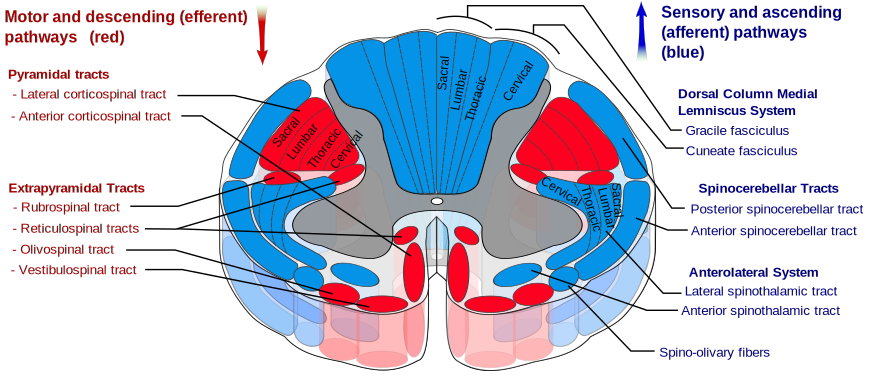
\includegraphics[width=0.7\textwidth,height=\textheight]{figures/cns/Spinal_cord_tracts_-_English.svg}

Figure 13.3:
\href{https://commons.wikimedia.org/wiki/File:Spinal_cord_tracts_-_English.svg}{Efferent
and afferent tracts of the spinal cord}

\begin{itemize}
\item
  Alpha motor neurons innervate extrafusal muscle fibers, which are the
  main force-generating component of a muscle. Their cell bodies are in
  the ventral horn of the spinal cord and they are sometimes called
  ventral horn cells. A single motor neuron may synapse with 150 muscle
  fibers on average. The motor neuron and all of the muscle fibers to
  which it connects is a motor unit. Motor units are split up into 3
  categories:

  \begin{itemize}
  \tightlist
  \item
    Slow (S) motor units stimulate small muscle fibers, which contract
    very slowly and provide small amounts of energy but are very
    resistant to fatigue, so they are used to sustain muscular
    contraction, such as keeping the body upright. They gain their
    energy via oxidative means and hence require oxygen. They are also
    called red fibers.
  \item
    Fast fatiguing (FF) motor units stimulate larger muscle groups,
    which apply large amounts of force but fatigue very quickly. They
    are used for tasks that require large brief bursts on energy, such
    as jumping or running. They gain their energy via glycolytic means
    and hence don't require oxygen. They are called white fibers.
  \item
    Fast fatigue-resistant motor units stimulate moderate-sized muscles
    groups that don't react as fast as the FF motor units, but can be
    sustained much longer (as implied by the name) and provide more
    force than S motor units. These use both oxidative and glycolytic
    means to gain energy.
  \end{itemize}
\end{itemize}

\hypertarget{neuromuscular-junction}{%
\subsection{\texorpdfstring{{13.5} Neuromuscular
Junction}{13.5 Neuromuscular Junction}}\label{neuromuscular-junction}}

A neuromuscular junction is a chemical synapse formed by the contact
between a motor neuron and a muscle fiber. It is the site in which a
motor neuron transmits a signal to a muscle fiber to initiate muscle
contraction. The sequence of events that results in the depolarization
of the muscle fiber at the neuromuscular junction begins when an action
potential is initiated in the cell body of a motor neuron, which is then
propagated by saltatory conduction along its axon toward the
neuromuscular junction. Once it reaches the terminal bouton, the action
potential causes a Ca\textsuperscript{2+} ion influx into the terminal
by way of the voltage-gated calcium channels. The Ca\textsuperscript{2+}
influx causes synaptic vesicles containing the neurotransmitter
acetylcholine to fuse with the plasma membrane, releasing acetylcholine
into the synaptic cleft between the motor neuron terminal and the
neuromuscular junction of the skeletal muscle fiber. Acetylcholine
diffuses across the synapse and binds to and activates nicotinic
acetylcholine receptors on the neuromuscular junction. Activation of the
nicotinic receptor opens its intrinsic sodium/potassium channel, causing
sodium to rush in and potassium to trickle out. As a result, the
sarcolemma reverses polarity and its voltage quickly jumps from the
resting membrane potential of -90mV to as high as +75mV as sodium
enters. The membrane potential then becomes hyperpolarized when
potassium exits and is then adjusted back to the resting membrane
potential. This rapid fluctuation is called the end-plate potential The
voltage-gated ion channels of the sarcolemma next to the end plate open
in response to the end plate potential. They are sodium and potassium
specific and only allow one through. This wave of ion movements creates
the action potential that spreads from the motor end plate in all
directions. If action potentials stop arriving, then acetylcholine
ceases to be released from the terminal bouton. The remaining
acetylcholine in the synaptic cleft is either degraded by active
acetylcholine esterase or reabsorbed by the synaptic knob and none is
left to replace the degraded acetylcholine.

\protect\hypertarget{fig:neuromuscularjunction}{}{}
\includegraphics[width=0.7\textwidth,height=\textheight]{figures/motor/1009_Motor_End_Plate_and_Innervation.jpg}

Figure 13.4:
\href{https://commons.wikimedia.org/wiki/File:1009_Motor_End_Plate_and_Innervation.jpg}{Structure
of neuromuscular junction.}

\hypertarget{muscle-contraction}{%
\subsubsection{\texorpdfstring{{13.5.1} Muscle
Contraction}{13.5.1 Muscle Contraction}}\label{muscle-contraction}}

Excitation--contraction coupling is the process by which a muscular
action potential in the muscle fiber causes the myofibrils to contract.
In skeletal muscle, excitation--contraction coupling relies on a direct
coupling between key proteins, the sarcoplasmic reticulum (SR) calcium
release channel (identified as the ryanodine receptor, RyR) and
voltage-gated L-type calcium channels (identified as dihydropyridine
receptors, DHPRs). DHPRs are located on the sarcolemma (which includes
the surface sarcolemma and the transverse tubules), while the RyRs
reside across the SR membrane. The close apposition of a transverse
tubule and two SR regions containing RyRs is described as a triad and is
predominantly where excitation--contraction coupling takes place.
Excitation--contraction coupling occurs when depolarization of skeletal
muscle cell results in a muscle action potential, which spreads across
the cell surface and into the muscle fiber's network of T-tubules,
thereby depolarizing the inner portion of the muscle fiber.
Depolarization of the inner portions activates dihydropyridine receptors
in the terminal cisternae, which are in close proximity to ryanodine
receptors in the adjacent sarcoplasmic reticulum. The activated
dihydropyridine receptors physically interact with ryanodine receptors
to activate them via foot processes (involving conformational changes
that allosterically activates the ryanodine receptors). As the ryanodine
receptors open, Ca\textsuperscript{2+} is released from the sarcoplasmic
reticulum into the local junctional space and diffuses into the bulk
cytoplasm to cause a calcium spark. Note that the sarcoplasmic reticulum
has a large calcium buffering capacity partially due to a
calcium-binding protein called calsequestrin. The near synchronous
activation of thousands of calcium sparks by the action potential causes
a cell-wide increase in calcium giving rise to the upstroke of the
calcium transient. The Ca\textsuperscript{2+} released into the cytosol
binds to Troponin C by the actin filaments, to allow crossbridge
cycling, producing force and, in some situations, motion. The
sarco/endoplasmic reticulum calcium-ATPase (SERCA) actively pumps
Ca\textsuperscript{2+} back into the sarcoplasmic reticulum. As
Ca\textsuperscript{2+} declines back to resting levels, the force
declines and relaxation occurs.

\hypertarget{sliding-filament-theory}{%
\subsubsection{\texorpdfstring{{13.5.2} Sliding filament
theory}{13.5.2 Sliding filament theory}}\label{sliding-filament-theory}}

The sliding filament theory describes a process used by muscles to
contract. It is a cycle of repetitive events that cause a thin filament
to slide over a thick filament and generate tension in the muscle. It
was independently developed by Andrew Huxley and Rolf Niedergerke and by
Hugh Huxley and Jean Hanson in 1954. Physiologically, this contraction
is not uniform across the sarcomere; the central position of the thick
filaments becomes unstable and can shift during contraction. However the
actions of elastic proteins such as titin are hypothesised to maintain
uniform tension across the sarcomere and pull the thick filament into a
central position.

\hypertarget{crossbridge-cycling}{%
\subsubsection{\texorpdfstring{{13.5.3} Crossbridge
cycling}{13.5.3 Crossbridge cycling}}\label{crossbridge-cycling}}

Crossbridge cycling is a sequence of molecular events that underlies the
sliding filament theory. A crossbridge is a myosin projection,
consisting of two myosin heads, that extends from the thick filaments.
Each myosin head has two binding sites: one for ATP and another for
actin. The binding of ATP to a myosin head detaches myosin from actin,
thereby allowing myosin to bind to another actin molecule. Once
attached, the ATP is hydrolyzed by myosin, which uses the released
energy to move into the ``cocked position'' whereby it binds weakly to a
part of the actin binding site. The remainder of the actin binding site
is blocked by tropomyosin. With the ATP hydrolyzed, the cocked myosin
head now contains ADP + Pi. Two Ca\textsuperscript{2+} ions bind to
troponin C on the actin filaments. The troponin-Ca\textsuperscript{2+}
complex causes tropomyosin to slide over and unblock the remainder of
the actin binding site. Unblocking the rest of the actin binding sites
allows the two myosin heads to close and myosin to bind strongly to
actin. The myosin head then releases the inorganic phosphate and
initiates a power stroke, which generates a force of 2 pN. The power
stroke moves the actin filament inwards, thereby shortening the
sarcomere. Myosin then releases ADP but still remains tightly bound to
actin. At the end of the power stroke, ADP is released from the myosin
head, leaving myosin attached to actin in a rigor state until another
ATP binds to myosin. A lack of ATP would result in the rigor state
characteristic of rigor mortis. Once another ATP binds to myosin, the
myosin head will again detach from actin and another crossbridges cycle
occurs.

Crossbridge cycling is able to continue as long as there are sufficient
amounts of ATP and Ca\textsuperscript{2+} in the cytoplasm. Termination
of crossbridge cycling can occur when Ca\textsuperscript{2+} is actively
pumped back into the sarcoplasmic reticulum. When Ca\textsuperscript{2+}
is no longer present on the thin filament, the tropomyosin changes
conformation back to its previous state so as to block the binding sites
again. The myosin ceases binding to the thin filament, and the muscle
relaxes. The Ca\textsuperscript{2+} ions leave the troponin molecule in
order to maintain the Ca\textsuperscript{2+} ion concentration in the
sarcoplasm. The active pumping of Ca\textsuperscript{2+} ions into the
sarcoplasmic reticulum creates a deficiency in the fluid around the
myofibrils. This causes the removal of Ca\textsuperscript{2+} ions from
the troponin. Thus, the tropomyosin-troponin complex again covers the
binding sites on the actin filaments and contraction ceases.

\protect\hypertarget{fig:crossbridge}{}{}
\includegraphics[width=0.7\textwidth,height=\textheight]{figures/motor/1008_Skeletal_Muscle_Contraction.jpg}

Figure 13.5:
\href{https://commons.wikimedia.org/wiki/File:1008_Skeletal_Muscle_Contraction.jpg}{Crossbridge
cycling and the molecular basis of muscle contraction.}

\hypertarget{the-stretch-reflex}{%
\subsubsection{\texorpdfstring{{13.5.4} The Stretch
Reflex}{13.5.4 The Stretch Reflex}}\label{the-stretch-reflex}}

\href{https://en.wikipedia.org/wiki/Wilhelm_Heinrich_Erb}{Wilhelm
Heinrich Erb} (1840--1921) and
\href{https://en.wikipedia.org/wiki/Carl_Friedrich_Otto_Westphal}{Carl
Friedrich Otto Westphal} (1833--1890) simultaneously reported the
patellar tendon or knee reflex in 1875 . The term knee-jerk was recorded
by Sir Michael Foster in his Textbook of physiology in 1877: ``Striking
the tendon below the patella gives rise to a sudden extension of the
leg, known as the knee-jerk.''

The patellar reflex or knee-jerk (myotatic) (monosynaptic) is a clinical
and classic example of the monosynaptic reflex arc. There is no
interneuron in the pathway leading to contraction of the quadriceps
muscle. Instead, the sensory neuron synapses directly on a motor neuron
in the spinal cord. However, there is an inhibitory interneuron used to
relax the antagonistic hamstring muscle (reciprocal innervation).

Striking of the patellar tendon with a reflex hammer just below the
patella stretches the muscle spindle in the quadriceps muscle. This
produces a signal which travels back to the spinal cord and synapses
(without interneurons) at the level of L3 in the spinal cord, completely
independent of higher centres. From there, an alpha motor neuron
conducts an efferent impulse back to the quadriceps femoris muscle,
triggering contraction. This contraction, coordinated with the
relaxation of the antagonistic flexor hamstring muscle causes the leg to
kick. This is a reflex of proprioception which helps maintain posture
and balance, allowing to keep one's balance with little effort or
conscious thought.

\hypertarget{the-motor-cortex}{%
\subsection{\texorpdfstring{{13.6} The Motor
Cortex}{13.6 The Motor Cortex}}\label{the-motor-cortex}}

The motor cortex is the region of the cerebral cortex involved in the
planning, control, and execution of voluntary movements. Classically the
motor cortex is an area of the frontal lobe located in the posterior
precentral gyrus immediately anterior to the central sulcus.

The motor cortex can be divided into three areas:

\begin{enumerate}
\def\labelenumi{\arabic{enumi}.}
\tightlist
\item
  The primary motor cortex is the main contributor to generating neural
  impulses that pass down to the spinal cord and control the execution
  of movement. However, some of the other motor areas in the brain also
  play a role in this function. It is located on the anterior
  paracentral lobule on the medial surface.
\item
  The premotor cortex is responsible for some aspects of motor control,
  possibly including the preparation for movement, the sensory guidance
  of movement, the spatial guidance of reaching, or the direct control
  of some movements with an emphasis on control of proximal and trunk
  muscles of the body. Located anterior to the primary motor cortex.
\item
  The supplementary motor area (or SMA), has many proposed functions
  including the internally generated planning of movement, the planning
  of sequences of movement, and the coordination of the two sides of the
  body such as in bi-manual coordination. Located on the midline surface
  of the hemisphere anterior to the primary motor cortex.
\end{enumerate}

Other brain regions outside the cerebral cortex are also of great
importance to motor function, most notably the cerebellum, the basal
ganglia, pedunculopontine nucleus and the red nucleus, as well as other
subcortical motor nuclei.

In 1870 Eduard Hitzig and Gustav Fritsch demonstrated that electrical
stimulation of certain parts of the dog brain resulted in muscular
contraction on the opposite side of the body.

A little later, in 1874, David Ferrier, working in the laboratory of the
West Riding Lunatic Asylum at Wakefield (at the invitation of its
director, James Crichton-Browne), mapped the motor cortex in the monkey
brain using electrical stimulation. He found that the motor cortex
contained a rough map of the body with the feet at the top (or dorsal
part) of the brain and the face at the bottom (or ventral part) of the
brain. He also found that when electrical stimulation was maintained for
a longer time, such as for a second, instead of being discharged over a
fraction of a second, then some coordinated, seemingly meaningful
movements could be caused, instead of only muscle twitches.

After Ferrier's discovery, many neuroscientists used electrical
stimulation to study the map of the motor cortex in many animals
including monkeys, apes, and humans.

One of the first detailed maps of the human motor cortex was described
in 1905 by Campbell. He did autopsies on the brains of amputees. A
person who had lost an arm would over time apparently lose some of the
neuronal mass in the part of the motor cortex that normally controls the
arm. Likewise, a person who had lost a leg would show degeneration in
the leg part of motor cortex. In this way the motor map could be
established. In the period between 1919 and 1936 others mapped the motor
cortex in detail using electrical stimulation, including the husband and
wife team Vogt and Vogt, and the neurosurgeon Foerster.

Perhaps the best-known experiments on the human motor map were published
by Penfield in 1937. Using a procedure that was common in the 1930s, he
examined epileptic patients who were undergoing brain surgery. These
patients were given a local anesthetic, their skulls were opened, and
their brains exposed. Then, electrical stimulation was applied to the
surface of the brain to map out the speech areas. In this way, the
surgeon would be able to avoid any damage to speech circuitry. The brain
focus of the epilepsy could then be surgically removed. During this
procedure, Penfield mapped the effect of electrical stimulation in all
parts of the cerebral cortex, including motor cortex.

Penfield is sometimes mistakenly considered to be the discoverer of the
map in motor cortex. It was discovered approximately 70 years before his
work. However, Penfield drew a picture of a human-like figure stretched
over the cortical surface and used the term ``homunculus'' (diminutive
of ``homo'', Latin for ``man'') to refer to it. It is perhaps for this
reason that his work has become so popular in neuroscience.

\hypertarget{the-supplementary-motor-cortex}{%
\subsubsection{\texorpdfstring{{13.6.1} The Supplementary Motor
Cortex}{13.6.1 The Supplementary Motor Cortex}}\label{the-supplementary-motor-cortex}}

\hypertarget{the-basal-ganglia-1}{}
\hypertarget{the-basal-ganglia}{%
\subsection{\texorpdfstring{{13.7} The Basal
Ganglia}{13.7 The Basal Ganglia}}\label{the-basal-ganglia}}

The basal ganglia (or basal nuclei) are a group of subcortical nuclei,
of varied origin, in the brains of vertebrates, including humans, which
are situated at the base of the forebrain and top of the midbrain. There
are some differences in the basal ganglia of primates. Basal ganglia are
strongly interconnected with the cerebral cortex, thalamus, and
brainstem, as well as several other brain areas. The basal ganglia are
associated with a variety of functions, including control of voluntary
motor movements, procedural learning, habit learning, eye movements,
cognition, and emotion.

The nomenclature of the basal ganglia system and its components has
always been problematic. Early anatomists, seeing the macroscopic
anatomical structure but knowing nothing of the cellular architecture or
neurochemistry, grouped together components that are now believed to
have distinct functions (such as the internal and external segments of
the globus pallidus), and gave distinct names to components that are now
thought to be functionally parts of a single structure (such as the
caudate nucleus and putamen).

The term ``basal'' comes from the fact that most of its elements are
located in the basal part of the forebrain. The term ganglia is a
misnomer: In modern usage, neural clusters are called ``ganglia'' only
in the peripheral nervous system; in the central nervous system they are
called ``nuclei''. For this reason, the basal ganglia are also
occasionally known as the ``basal nuclei''.

The main components of the basal ganglia -- as defined functionally --
are the striatum; both dorsal striatum (caudate nucleus and putamen) and
ventral striatum (nucleus accumbens and olfactory tubercle), globus
pallidus, ventral pallidum, substantia nigra, and subthalamic nucleus.
Each of these components has a complex internal anatomical and
neurochemical organization. The largest component, the striatum (dorsal
and ventral), receives input from many brain areas beyond the basal
ganglia, but only sends output to other components of the basal ganglia.
The pallidum receives input from the striatum, and sends inhibitory
output to a number of motor-related areas. The substantia nigra is the
source of the striatal input of the neurotransmitter dopamine, which
plays an important role in basal ganglia function. The subthalamic
nucleus receives input mainly from the striatum and cerebral cortex, and
projects to the globus pallidus.

Popular theories implicate the basal ganglia primarily in action
selection -- in helping to decide which of several possible behaviors to
execute at any given time. In more specific terms, the basal ganglia's
primary function is likely to control and regulate activities of the
motor and premotor cortical areas so that voluntary movements can be
performed smoothly. Experimental studies show that the basal ganglia
exert an inhibitory influence on a number of motor systems, and that a
release of this inhibition permits a motor system to become active. The
``behavior switching'' that takes place within the basal ganglia is
influenced by signals from many parts of the brain, including the
prefrontal cortex, which plays a key role in executive functions.

The basal ganglia are of major importance for normal brain function and
behaviour. Their dysfunction results in a wide range of neurological
conditions including disorders of behaviour control and movement. Those
of behaviour include Tourette syndrome, obsessive--compulsive disorder,
and addiction. Movement disorders include, most notably Parkinson's
disease, which involves degeneration of the dopamine-producing cells in
the substantia nigra, Huntington's disease, which primarily involves
damage to the striatum, dystonia, and more rarely hemiballismus. The
basal ganglia have a limbic sector whose components are assigned
distinct names: the nucleus accumbens, ventral pallidum, and ventral
tegmental area (VTA). There is considerable evidence that this limbic
part plays a central role in reward learning as well as cognition and
frontal lobe functioning, via the mesolimbic pathway from the VTA to the
nucleus accumbens that uses the neurotransmitter dopamine, and the
mesocortical pathway. A number of highly addictive drugs, including
cocaine, amphetamine, and nicotine, are thought to work by increasing
the efficacy of this dopamine signal. There is also evidence implicating
overactivity of the VTA dopaminergic projection in schizophrenia.

The basal ganglia form a fundamental component of the cerebrum. In
contrast to the cortical layer that lines the surface of the forebrain,
the basal ganglia are a collection of distinct masses of gray matter
lying deep in the brain not far from the junction of the thalamus. They
lie to the side of and surround the thalamus. Like most parts of the
brain, the basal ganglia consist of left and right sides that are
virtual mirror images of each other.

\hypertarget{the-cortico-basal-ganglia-thalamo-cortical-loop}{%
\subsection{\texorpdfstring{{13.8} The Cortico-Basal
Ganglia-Thalamo-Cortical
Loop}{13.8 The Cortico-Basal Ganglia-Thalamo-Cortical Loop}}\label{the-cortico-basal-ganglia-thalamo-cortical-loop}}

The cortico-basal ganglia-thalamo-cortical loop (CBGTC loop) is a system
of neural circuits in the brain. The loop involves connections between
the cortex, the basal ganglia, the thalamus, and back to the cortex. It
is of particular relevance to hyperkinetic and hypokinetic movement
disorders, such as Parkinson's disease and Huntington's disease, as well
as to mental disorders of control, such as attention deficit
hyperactivity disorder (ADHD), obsessive--compulsive disorder (OCD), and
Tourette syndrome.

The CBGTC loop primarily consists of modulatory dopaminergic projections
from the pars compacta of the substantia nigra, and ventral tegmental
area as well as excitatory glutamatergic projections from the cortex to
the striatum, where these projections form synapses with excitatory and
inhibitory pathways that relay back to the cortex.

The two major input structures of the circuit are the striatum and the
subthalamic nucleus (STN). The striatum receives inputs from both the
cortex and the pars compacta of the substantia nigra (SNc), while the
STN only receives cortical inputs.

Two pathways emerge from the striatum. One pathway is called the
indirect (or NoGo) pathway and is inhibitory. This projects to and
inhibits the globus pallidus externus (GPe), resulting in the
disinhibition of the globus pallidus internus (GPi), leading to
inhibition of the thalamus. This pathway also, as a result of inhibiting
the GPe, disinhibits the subthalamic nucleus, which results in
excitation of the GPi, and therefore inhibition of the thalamus.

The second pathway, is called the direct (or Go) pathway and is
excitatory. This pathway inhibits the GPi, resulting in the
disinhibition of the thalamus. The direct pathway mostly consists of
monosynaptic connections driven by dopamine receptor D1, adenosine A1
receptor, and muscarinic acetylcholine receptor M4, while the indirect
pathway relies on connections driven by dopamine receptor D2, adenosine
A2A receptor, and muscarinic acetylcholine receptor M1.

\protect\hypertarget{fig:basalcircuits}{}{}
\includegraphics[width=0.7\textwidth,height=\textheight]{figures/motor/Basal_ganglia_circuits.svg}

Figure 13.6:
\href{https://commons.wikimedia.org/wiki/File:Basal_ganglia_circuits.svg}{Circuits
of the basal ganglia.} Picture shows 2 coronal slices that have been
superimposed to include the involved basal ganglia structures. + and -
signs at the point of the arrows indicate respectively whether the
pathway is excitatory or inhibitory in effect. Green arrows refer to
excitatory glutamatergic pathways, red arrows refer to inhibitory
GABAergic pathways and turquoise arrows refer to dopaminergic pathways
that are excitatory on the direct pathway and inhibitory on the indirect
pathway. Note that dis-inhibitory pathways in effect are excitatory on
the feedback to the cortex, while dis-dis-inhibitory pathways in effect
are inhibitory. See en:Basal ganglia\#Connections

The CBGTC loop has been implicated in many diseases. For example, in
Parkinson's disease, degeneration of dopaminergic neurons leading to
decreased activity of the excitatory pathway is thought to result in
hypokinesia, and in Huntington's disease, degeneration of GABAergic
neurons driving the inhibitory pathway is thought to result in the jerky
body movements. The co-degeneration of limbic projections along with
motor projections may result in many of the psychiatric symptoms of
these primarily motor illnesses.

\hypertarget{the-pyramidal-motor-system}{%
\subsection{\texorpdfstring{{13.9} The Pyramidal Motor
System}{13.9 The Pyramidal Motor System}}\label{the-pyramidal-motor-system}}

The pyramidal motor system, also called the pyramidal tract or the
corticospinal tract, start in the motor center of the cerebral cortex.
There are upper and lower motor neurons in the corticospinal tract. The
motor impulses originate in the giant pyramidal cells or Betz cells of
the motor area; i.e., precentral gyrus of cerebral cortex. These are the
upper motor neurons (UMN) of the corticospinal tract. The axons of these
cells pass in the depth of the cerebral cortex to the corona radiata and
then to the internal capsule passing through the posterior branch of
internal capsule and continue to descend in the midbrain and the medulla
oblongata. In the lower part of Medulla oblongata 80 to 85\% of these
fibers decussate (pass to the opposite side) and descend in the white
matter of the lateral funiculus of the spinal cord on the opposite side.
The remaining 15 to 20\% pass to the same side. Fibers for the
extremities (limbs) pass 100\% to the opposite side. The fibers of the
corticospinal tract terminate at different levels in the anterior horn
of the grey matter of the spinal cord. Here the lower motor neurons
(LMN) of the corticospinal cord are located. Peripheral motor nerves
carry the motor impulses from the anterior horn to the voluntary
muscles.

The pyramidal tracts include both the corticobulbar tract and the
corticospinal tract. These are aggregations of efferent nerve fibers
from the upper motor neurons that travel from the cerebral cortex and
terminate either in the brainstem (corticobulbar) or spinal cord
(corticospinal) and are involved in the control of motor functions of
the body.

The corticobulbar tract conducts impulses from the brain to the cranial
nerves. These nerves control the muscles of the face and neck and are
involved in facial expression, mastication, swallowing, and other
functions.

The corticospinal tract conducts impulses from the brain to the spinal
cord. It is made up of a lateral and anterior tract. The corticospinal
tract is involved in voluntary movement. The majority of fibres of the
corticospinal tract cross over in the medulla oblongata, resulting in
muscles being controlled by the opposite side of the brain. The
corticospinal tract also contains the axons of Betz cells (the largest
pyramidal cells) located in the primary motor cortex.

The pyramidal tracts are named because they pass through the pyramids of
the medulla oblongata. The corticospinal fibers when descending from the
internal capsule to the brain stem, converge to a point from multiple
directions giving the impression of an inverted pyramid.

The myelination of the pyramidal fibres is incomplete at birth and
gradually progresses in cranio-caudal direction and thereby
progressively gaining functionality. Most of the myelination is complete
by two years of age and thereafter it progresses very slowly in
cranio-caudal direction up to twelve years of age.

\hypertarget{the-corticospinal-tract-1}{}
\hypertarget{the-corticospinal-tract}{%
\subsubsection{\texorpdfstring{{13.9.1} The Corticospinal
Tract}{13.9.1 The Corticospinal Tract}}\label{the-corticospinal-tract}}

Nerve fibres in the corticospinal tract originate from pyramidal cells
in layer V of the cerebral cortex. Fibres arise from the primary motor
cortex (about 30\%), supplementary motor area and the premotor cortex
(together also about 30\%), and the somatosensory cortex, parietal lobe,
and cingulate gyrus supplies the rest. The cells have their bodies in
the cerebral cortex, and the axons form the bulk of the pyramidal
tracts. The nerve axons travel from the cortex through the posterior
limb of internal capsule, through the cerebral peduncle and into the
brainstem and anterior medulla oblongata. Here they form two prominences
called the medulla oblongatary pyramids. Below the prominences, the
majority of axons cross over to the opposite side from which they
originated, known as decussation. The axons that cross over move to the
outer part of the medulla oblongata and form the lateral corticospinal
tract, whereas the fibres that remain form the anterior corticospinal
tract. About 80\% of axons cross over and form the lateral corticospinal
tract; 10\% do not cross over and join the tract, and 10\% of fibres
travel in the anterior corticospinal tract.

The nerve axons traveling down the tract are the efferent nerve fibers
of the upper motor neurons. These axons travel down the tracts in the
white matter of the spinal cord until they reach the vertebral level of
the muscle that they will innervate. At this point, the axons synapse
with lower motor neurons. The majority of axons do not directly synapse
with lower motor neurons, but instead synapse with an interneuron that
then synapses with a lower motor neuron. This generally occurs in the
anterior grey column. Nerve axons of the lateral corticospinal tract
that did not cross over in the medulla oblongata do so at the level of
the spinal cord they terminate in.

These tracts contain more than 1 million axons and the majority of the
axons are myelinated. The corticospinal tracts myelinate largely during
the first and second years after birth. The majority of nerve axons are
small (\textless4μm) in diameter. About 3\% of nerve axons have a much
larger diameter (16μm) and arise from Betz cells, mostly in the leg area
of the primary motor cortex. These cells are notable because of their
rapid conduction rate, over 70m/sec, the fastest conduction of any
signals from the brain to the spinal cord.

\hypertarget{the-corticobulbar-tract-1}{}
\hypertarget{the-corticobulbar-tract}{%
\subsubsection{\texorpdfstring{{13.9.2} The Corticobulbar
Tract}{13.9.2 The Corticobulbar Tract}}\label{the-corticobulbar-tract}}

Fibres from the ventral motor cortex travel with the corticospinal tract
through the internal capsule, but terminate in a number of locations in
the midbrain (cortico-mesencephalic tract), pons (Corticopontine tract),
and medulla oblongata (cortico-bulbar tract). The upper motor neurons of
the corticobulbar tract synapse with interneurons or directly with the
lower motor neurons located in the motor cranial nerve nuclei, namely
oculomotor, trochlear, motor nucleus of the trigeminal nerve, abducens,
facial nerve and accessory and in the nucleus ambiguus to the
hypoglossal, vagus and accessory nerves. These nuclei are supplied by
nerves from both sides of the brain, with the exception of the parts of
the facial nerve that control muscles of the lower face. These muscles
are only innervated by nerves from the contralateral (opposite) side of
the cortex.

The nerves within the corticospinal tract are involved in movement of
muscles of the body. Because of the crossing-over of fibres, muscles are
supplied by the side of the brain opposite to that of the muscle. The
nerves within the corticobulbar tract are involved in movement in
muscles of the head. They are involved in swallowing, phonation, and
movements of the tongue. By virtue of involvement with the facial nerve,
the corticobulbar tract is also responsible for transmitting facial
expression. With the exception of lower muscles of facial expression,
all functions of the corticobulbar tract involve inputs from both sides
of the brain.

\hypertarget{the-extrapyramidal-motor-system}{%
\subsection{\texorpdfstring{{13.10} The Extrapyramidal Motor
System}{13.10 The Extrapyramidal Motor System}}\label{the-extrapyramidal-motor-system}}

The extrapyramidal motor system consists of motor-modulation systems,
particularly the basal ganglia and cerebellum. The system is called
extrapyramidal to distinguish it from the tracts of the motor cortex
that reach their targets by traveling through the pyramids of the
medulla.

Extrapyramidal tracts are chiefly found in the reticular formation of
the pons and medulla, and target lower motor neurons in the spinal cord
that are involved in reflexes, locomotion, complex movements, and
postural control. These tracts are in turn modulated by various parts of
the central nervous system, including the nigrostriatal pathway, the
basal ganglia, the cerebellum, the vestibular nuclei, and different
sensory areas of the cerebral cortex. All of these regulatory components
can be considered part of the extrapyramidal system, in that they
modulate motor activity without directly innervating motor neurons.

The extrapyramidal tracts include parts of the following:

\begin{itemize}
\tightlist
\item
  rubrospinal tract
\item
  pontine reticulospinal tract
\item
  medullary reticulospinal tract
\item
  lateral vestibulospinal tract
\item
  tectospinal tract
\end{itemize}

In terms of anatomy, the basal ganglia are divided into four distinct
structures, depending on how superior or rostral they are (in other
words depending on how close to the top of the head they are): Two of
them, the striatum and the pallidum, are relatively large; the other
two, the substantia nigra and the subthalamic nucleus, are smaller. In
the illustration to the right, two coronal sections of the human brain
show the location of the basal ganglia components. Of note, and not seen
in this section, the subthalamic nucleus and substantia nigra lie
farther back (posteriorly) in the brain than the striatum and pallidum.

\href{the-gustatory-system.html}{\emph{}}
\href{major-diseases-of-the-nervous-system.html}{\emph{}}
